% !TEX root = main.tex
\appendix

\chapter{News articles}\label{App:A}
The project spawned several news articles and interviews. Below are multiple of these attached, along with a picture of Alex Nørgaard and I from our appearance on Go' Morgen Danmark.

		\begin{figure}
			\centering
			\caption{Alex Nørgaard, Mikkel Kryger and Carl-Emil Grøn on Go' Morgen Danmark on TV2}
			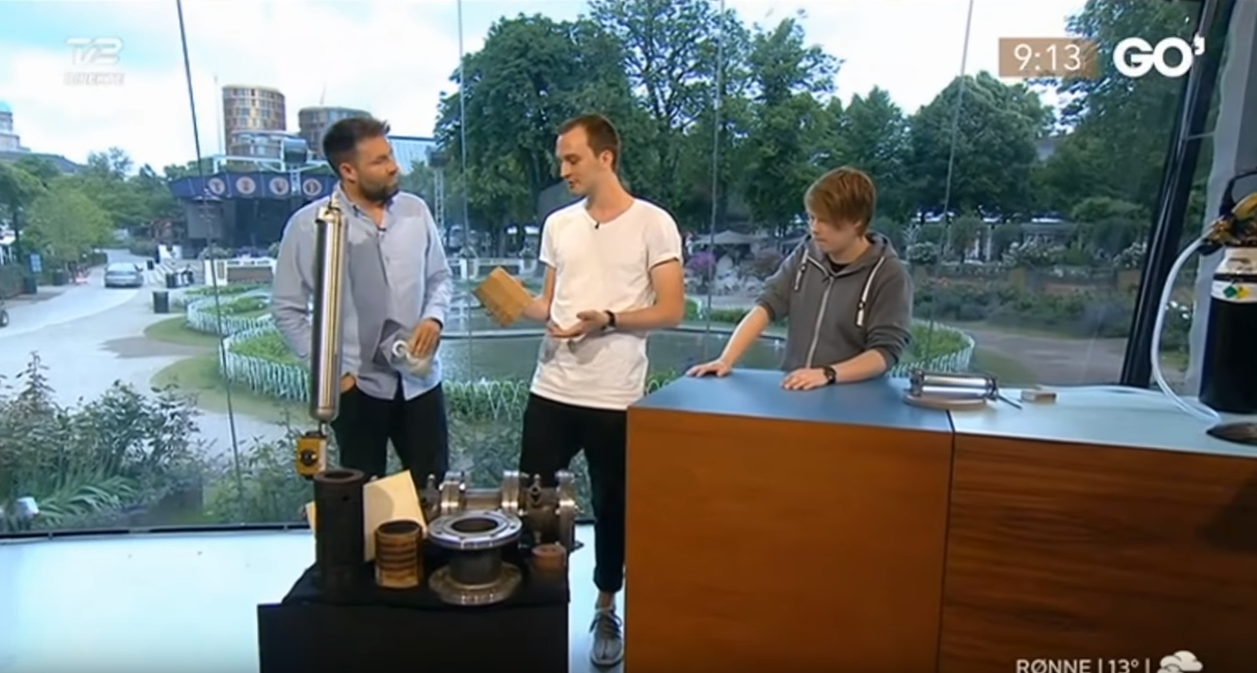
\includegraphics[width=\textwidth]{carlontv}
		\end{figure}

Go' Morgen DK on TV2:\\
\url{https://www.youtube.com/watch?v=YS0iT8jm7lo}
Peter Madsen's blogpost on Ingeniøren:\\ \url{https://ing.dk/blog/katalytisk-aktivt-besoeg-183974}\\
P4's interview of Alex Nørgaard:\\ \url{https://drive.google.com/file/d/0B0FJw8vW3gGmY2J5SDVlcE4zaFU/view}\\
AU Engineering news' article:\\ \url{http://ingenioer.au.dk/aktuelt/nyheder/nyhed/artikel/studerende-vil-sende-raket-ud-i-rummet/}




\chapter{Rocket Logbook} \label{App:B}

Below is a logbook with directions on how the rocket was fired, along with some general firing guidelines for future groups. Several notes are found below that contain thoughts, notes and events that happened during the testing schedule. 

	\section{Day 1}

		The test setup consists of the rocket engine with several piezoelectric and piezoresistive pressure sensors, as well as a force sensor at the back. The pressure sensors sit at various sites on the rocket, allowing us to detect any pressure waves travelling through the chamber, and measuring the rocket's pressure throughout the firing. The force sensor (henceforth mentioned as ForceLink) measures the rocket's thrust.

		The equipment is set up with LabVIEW, which Gorm spent most of the first day configuring. The rocket setup was tested on day 1, otherwise, the day consisted mostly of setting up the tent and establishing a remote connection to a new computer and installing the necessary programs.

	\section{Day 2}

		\begin{figure}
			\centering
			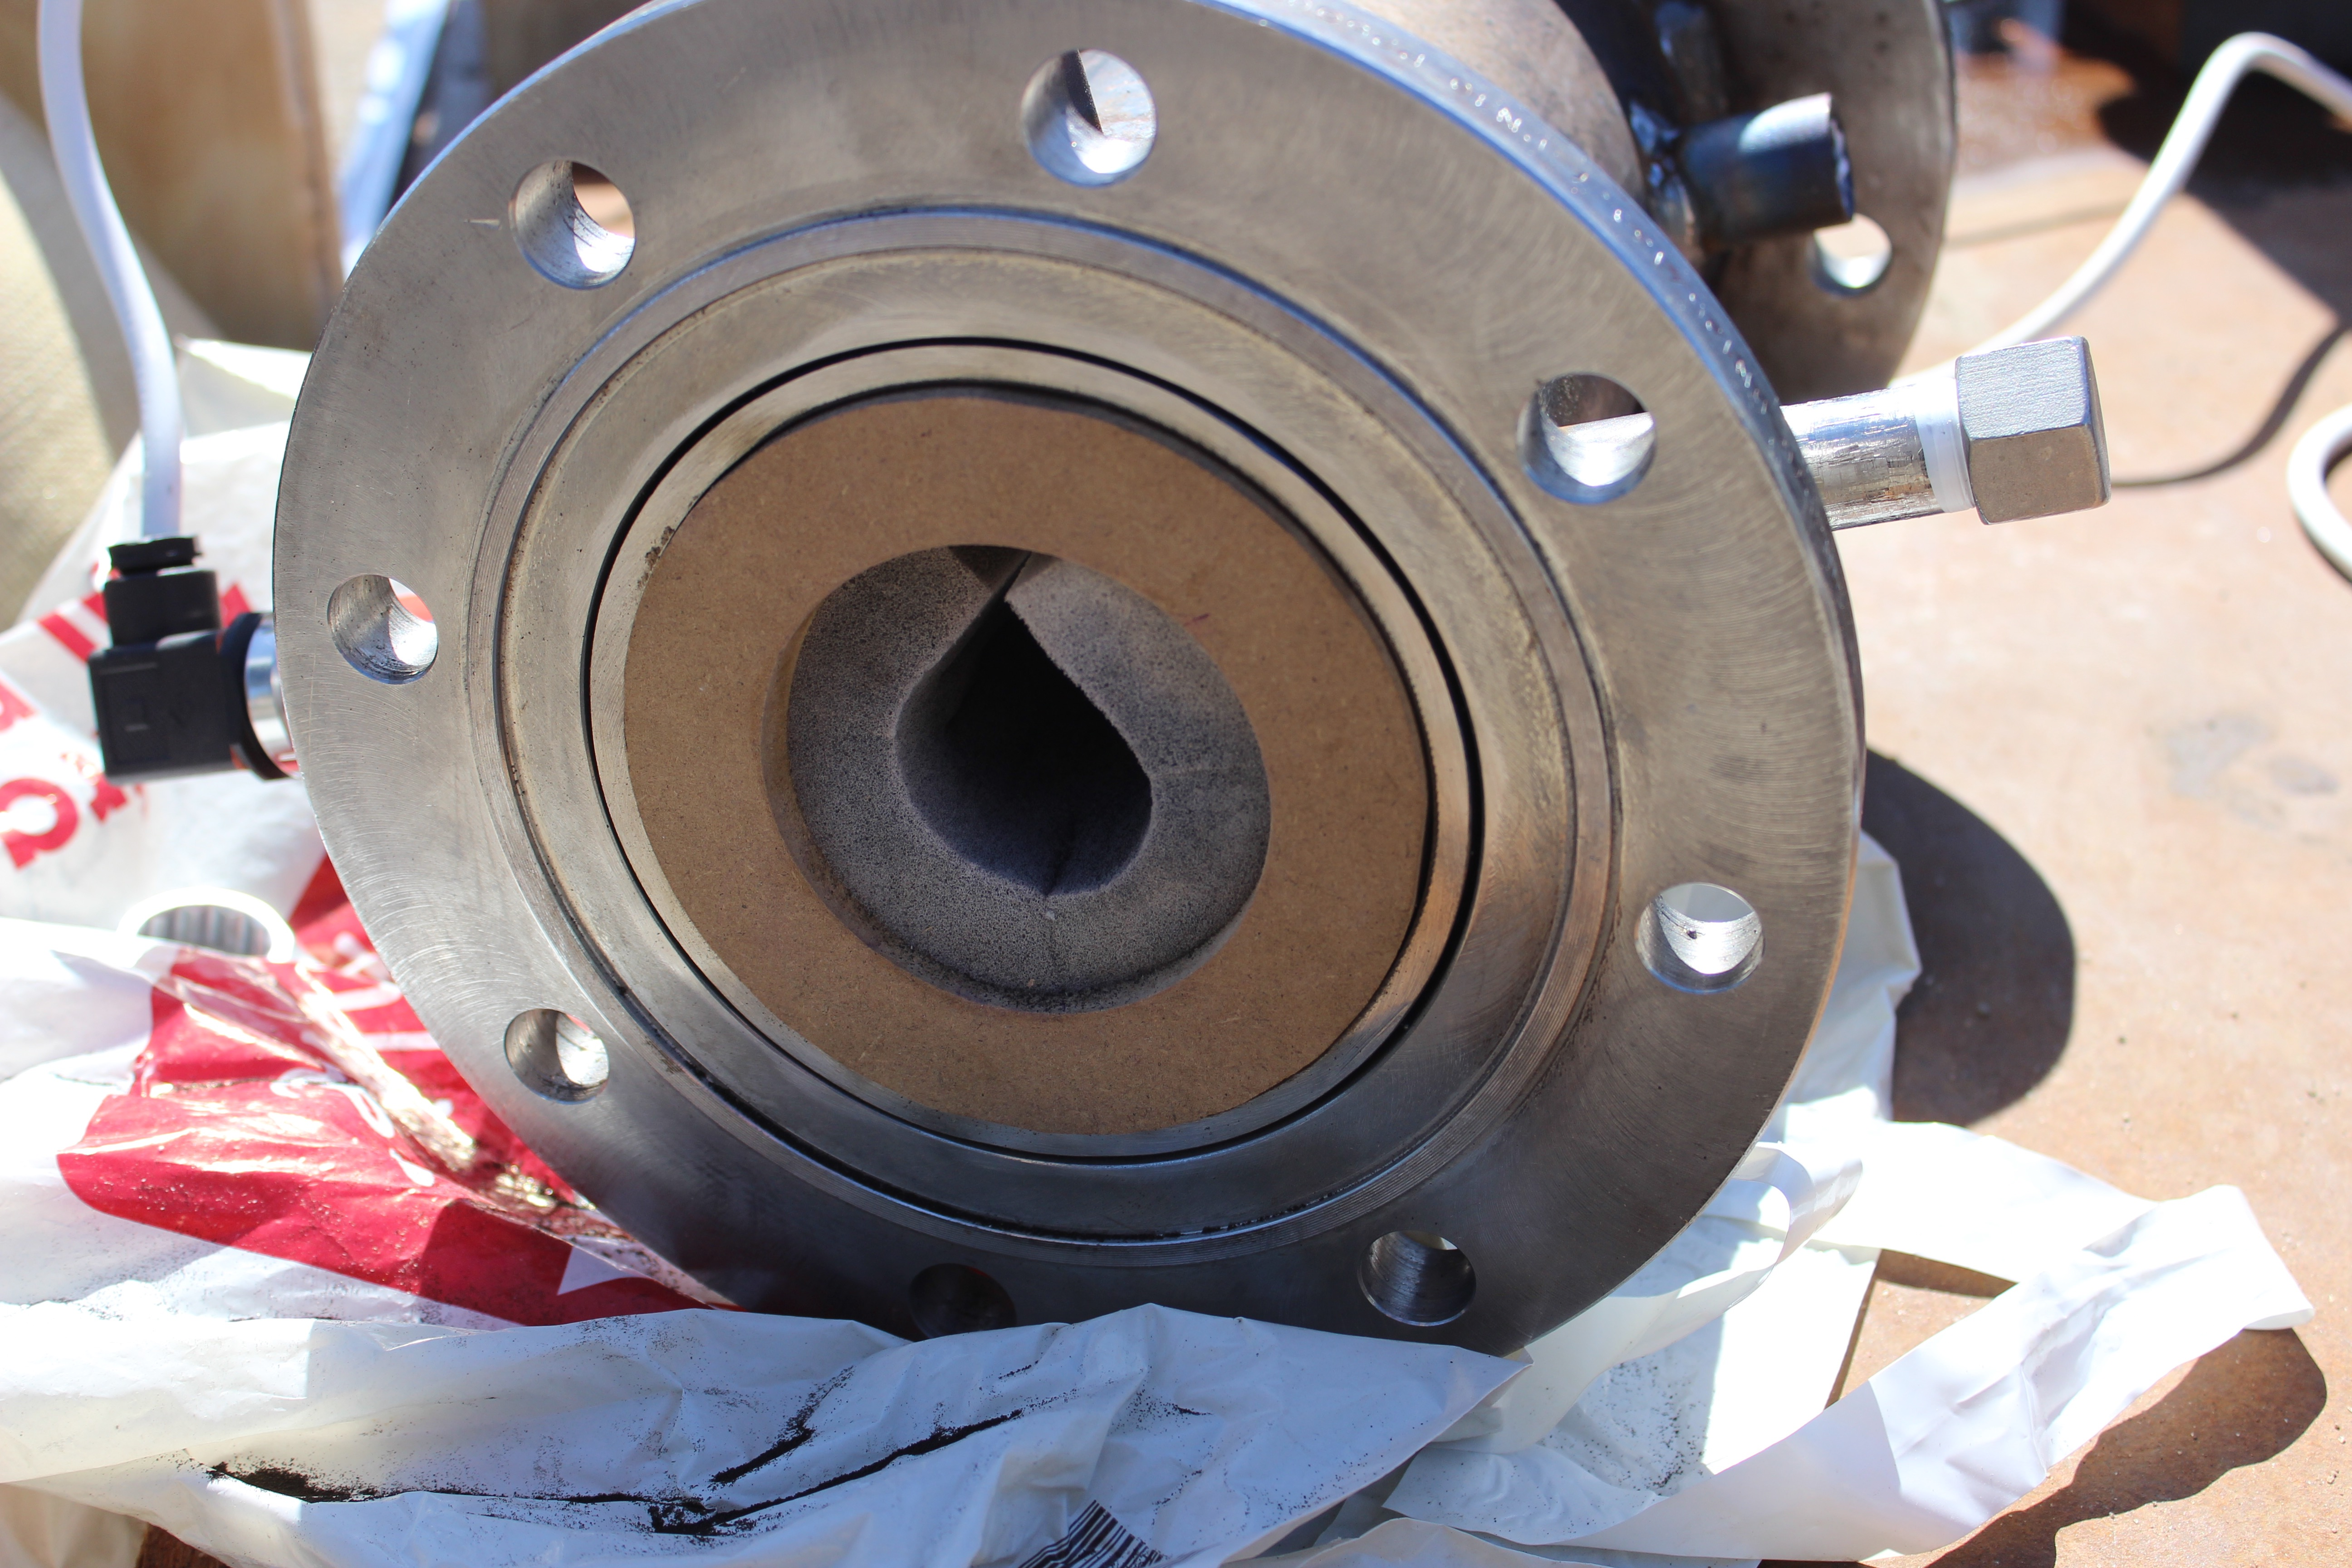
\includegraphics[width=\textwidth]{decompchamber}
			\caption{Foam permeated with \chem{KMnO_4} dust inserted into the decomposition chamber, inside a tube of MDF, in order to avoid accumulation of liquid \chem{H_2 O_2}}
			\label{fig:kmno4foam}
		\end{figure}

		Day 2 started early with preliminary water tests at 12:13, 12:33, 12:57 and 13:21. Two injectors, a low-flow and a high-flow, were brought along and tests of both ensued. Following the preliminary water tests, the rocket chambers were assembled and foam permeated with \chem{KMnO_4} was prepared and inserted into the decomposition chamber, as seen in figure \ref{fig:kmno4foam}. Initial rocket test started almost two hours after the final water test at 15:20 with $\SI{1.5}{\liter}$ of \chem{H_2 O_2} at $\SI{24}{\bar}$ pressure. After the test, the stand was quite smokey as the rocket flanges were \emph{not} tightened correctly and an O-ring was missing. A leak between the grain's chamber and the after-burn chamber seared the underside of the protective casing, thankfully without harming any of the measurement equipment. After the small upset, three additional tests were carried out. \fxnote{EVT. Lav tabel over tests i stedet for at skrive det}

		The three first tests were all done with the low-flow nozzle with a total radius of $\SI{1.5}{\milli \metre}$ per injector hole, of which there were three. The final tests were carried out with the large injector with hole radii of $\SI{2}{\milli \metre}$. The second test happened at 17:22 with a \chem{H_2 O_2} pressure of $\SI{24}{\bar}$, the next at 18:32 with $\SI{31}{bar}$. The final test was done at 20:19, with a \chem{H_2 O_2} pressure of $\si{31}{bar}$, with the high-flow nozzle.

		All tests were done with the same hexagonal patterned grain, with masses pre- and postburn noted.

		The day concluded with Peter Madsen using our test rig to test his own rocket based on a catalytic pack, with no combustion present.

		The firing procedure was meticulously planned out, in order to avoid any eventual dangers. Thus, including a such list is essential for future rocketeers:

\section{Firing Procedure}
	Launching the rocket requires several crucial steps in order to safely ignite the engine. Safety is the number one priority, thus, a stepwise checklist is necessary.

PRELAUNCH
\begin{enumerate}
  \itemsep0em
  \item Insert grain
  \item Insert foam permeated with \chem{KMnO_4}
  \item Assemble rocket chambers
  \item Establish remote access to control computer
  \item Ensure measurement options are correct
  \item Check signal and restart ManuWare
  \item Create new data-log file
\end{enumerate}
ALL CLEAR AREA EXCEPT FUEL RESPONSIBLE PERSON
\begin{enumerate}
  \itemsep0em
  \item Equip \chem{H_2 O_2} safety equipment
  \item Fill tank with \chem{H_2 O_2}
  \item Pressurize tank
  \item CLEAR THE AREA
  \item Start data-collection and cameras
  \item Arm the rocket
  \item Fire the rocket
  \item Stop data-collection and cameras
  \item Remove external pressure compressor
  \item Depressurize tank
  \item Area is safe
\end{enumerate}

	Peter Madsen and his assistant Stefan Eisenknappl are the only two people present when loading the rocket with \chem{H_2 O_2}. The procedure is executed from start to end at each launch, and has several areas where it can be improved if time permits.

\chapter{Enlarged Flowchart} \label{App:C}

	In order to assist rewriting the code from scratch, a more complex and complete version of the flowchart can be found below. Listed to the right of the previously centered posts are equations used to calculate the various variables. Full code can be found at \url{https://github.com/carlegroen/bachelors_degree} under the Rocket Model folder. The current, most stable and best working version is called: "\emph{IsentropicidentitymodelV3.m}".

		\begin{figure}
			\centering
			\includegraphics[width=0.75\textwidth]{flowchartfull}
			\caption{Full flowchart with equations used to calculate the various variables.}
			\label{fig:flowchartfull}
		\end{figure}